\documentclass[a4 paper, 11 pt]{article}

\usepackage[left=0.5in, right=0.5in, top=1in, bottom=1in]{geometry}
\usepackage{fancyhdr}
\usepackage{graphicx}
\usepackage{amsthm}
\usepackage{amsmath}
\usepackage{amssymb}
\usepackage{multirow}
\usepackage{graphicx}

\begin{document}
\begin{titlepage}
\begin{center}
\textsc{\huge Regression Homework 5} \\ [0.5cm]
\textsc{\huge Three Major Japanese Automakers--Price of Automobile}\\ [1.5cm]
\textsc{\large Janet Ye: jy1151} \\
\vfill
{\large \today}
\end{center}
\end{titlepage}

\section{Introduction}
The three major Japanese automakers are Toyota, Honda, and Nissan. What determines the price of a Japanese automobile? Naturally, one would think that the types--with levels car, Truck, SUV, and the Miles Per Gallon (MPG) are the main factors that affect the prices of automobile. In this analysis, we examine the relationship between the prices of the cars and the two predictor variables--type and MPG.
\section{The Data}
The data are manually recorded from the automakers' websites. All cars in the data set are gasoline fueled. We excluded hybrid models, since Toyota has hybrid cars and hybrid SUV, but Honda and Civic have hybrid cars only. The prices recorded down are manufactures suggested price. For MPG, I averaged city and highway MPG.

Below are a quick summary statistics.
\begin{center}
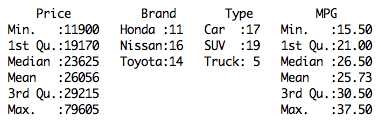
\includegraphics[scale=0.6]{sum} \\
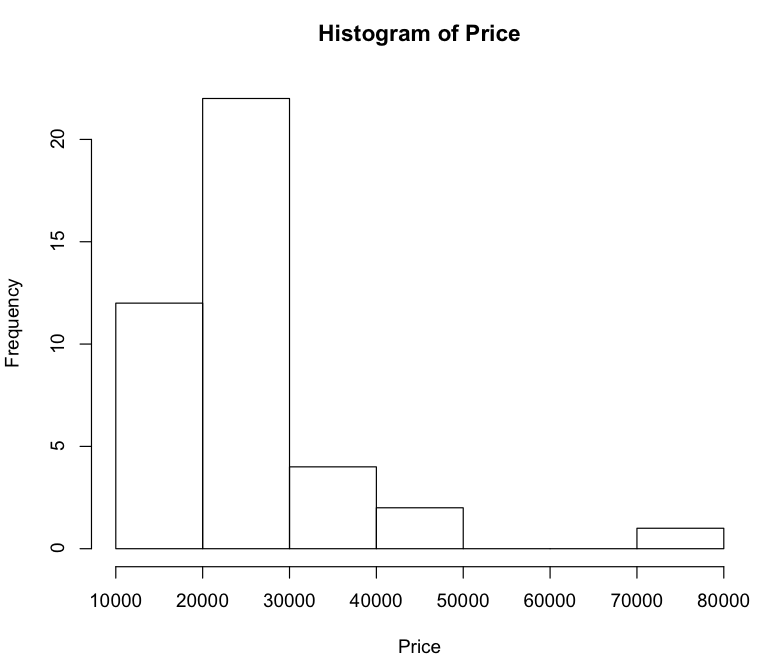
\includegraphics[scale=0.3]{histprice}
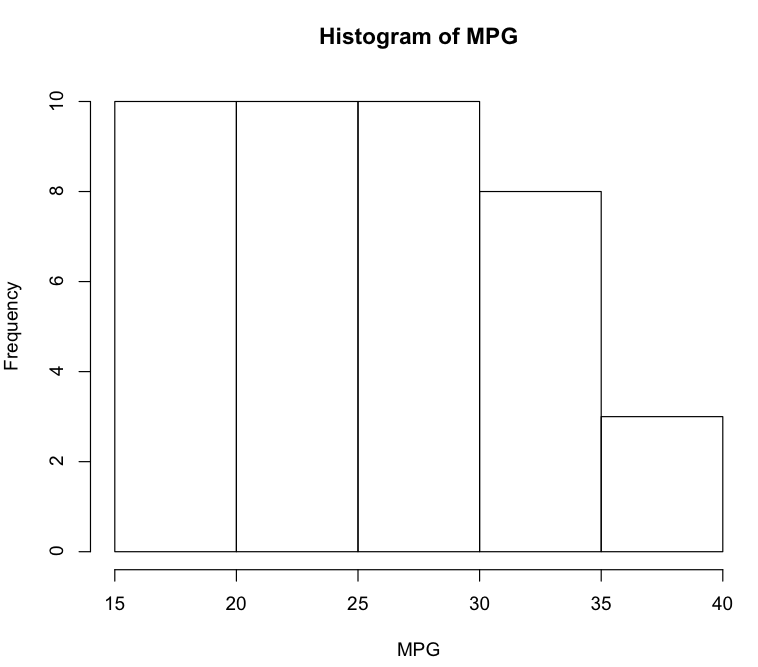
\includegraphics[scale=0.3]{histmpg}
\end{center}
The prices of the cars are skewed right. We will therefore work in the log scale. The histogram of MPG looks okay.

Below is the histogram of logged price. The plot looks more normal.
\begin{center}
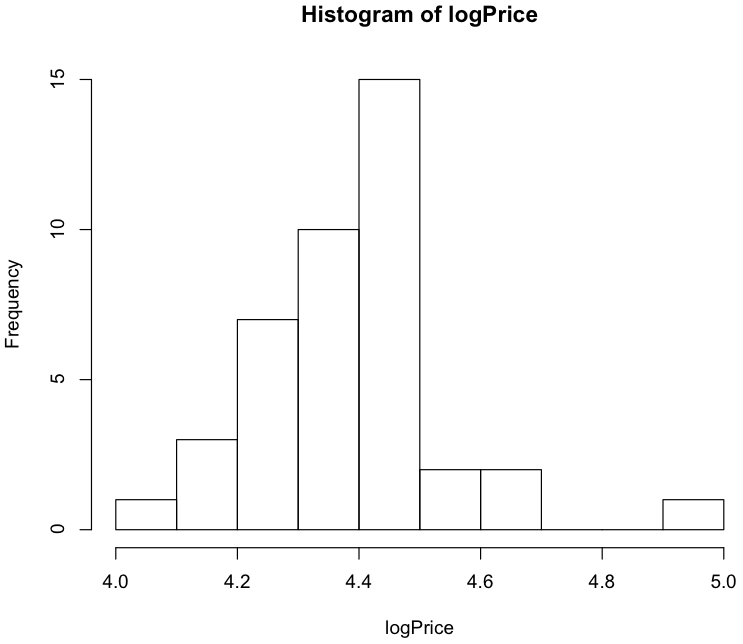
\includegraphics[scale=0.3]{histlogprice}
\end{center}
Side-by-side box plots show that types of vehicles have a marginal effect on the price, with car having the lowest mean price, trucks slightly lower than SUVs.

There also appears to be a moderate to strong, negative, linear relationship between MPG and logged Price. This makes sense as higher MPG vehicles are mostly cars, while lower MPG vehicles are SUVs and trucks. Cars generally cost less compare to SUVs and trucks.
\begin{center}
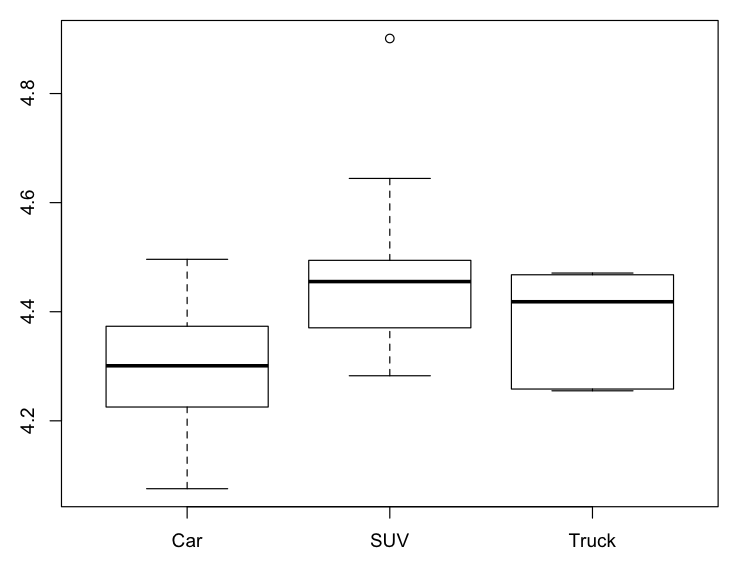
\includegraphics[scale=0.3]{boxtype}
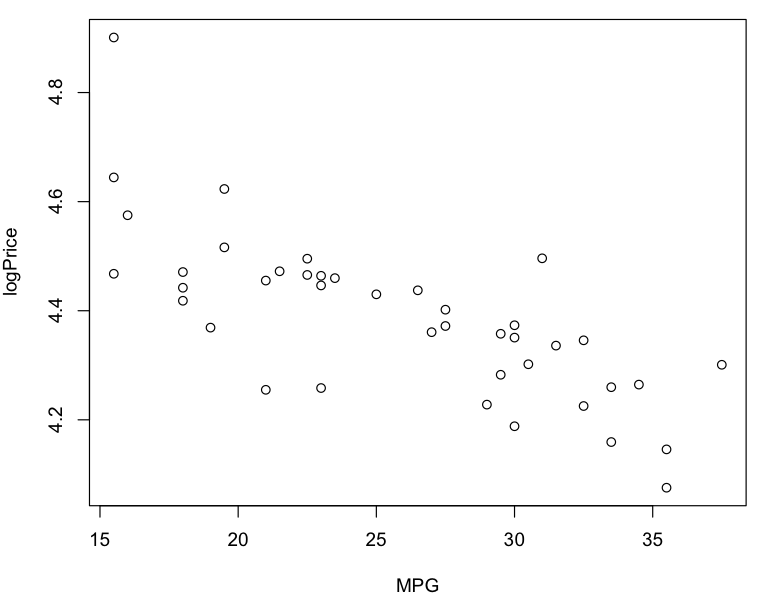
\includegraphics[scale=0.3]{pricempg}
\end{center}
\section{ANCOVA Model}
The ANCOVA model relates types of the automobile and MPG to logged prices of the automobile. Here is the output.
\begin{center}
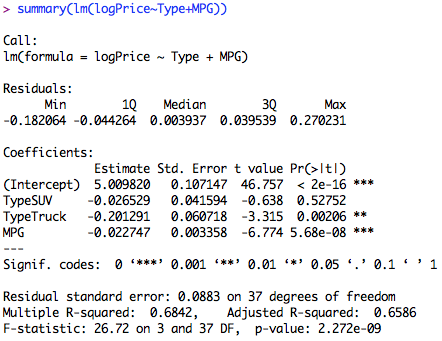
\includegraphics[scale=0.5]{d1lm}\\
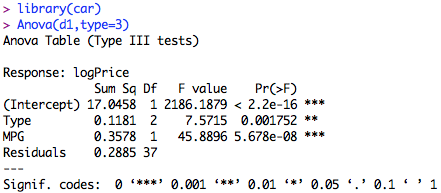
\includegraphics[scale=0.5]{d1ls}
\end{center}
Both types of the automobile and MPG are significant predictors for logged Price. They have F values 7.57 and 45.99, respectively; $p$-values are below any reasonable $\alpha$. The output shows that there is a negative relationship between MPG and logged Price, with 10 additional MPG associated with a decrease in logged Price of $(10)(0.022747) = \$0.22747$, that is, 10 additional MPG is associated with multiplying the Price by $10^{-0.22747} = \$0.592284$, or a reduction in price of 69\%, given the type of automobile is held fixed.

The following output gives the the least squares means.
\begin{center}
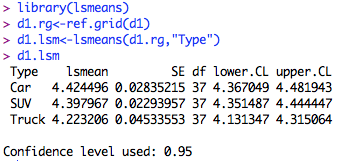
\includegraphics[scale=0.55]{d1lsm}
\end{center}
The entries under Least Squares Means for logged price show that given MPG, trucks cost the least, followed by SUVs, and cars cost the most. The difference between trucks and SUVs is $4.397967 - 4.223206 = 0.174761$, which means that given that two automobile have the same MPG, the expected price of an SUV is a multiplicative factor of $10^{0.174761} = 1.49541$, that is, 49.54\%, higher than that of a truck.

The difference between cars and SUVs is $4.424496 - 4.397967 = 0.026529$, which means that given that two automobile have the same MPG, the expected price of a car is a multiplicative factor of $10^{0.026529} = 1.062990$, that is, 6.3\%, higher than that of an SUV.

The difference between cars and trucks is $4.424496 - 4.223206 = 0.20129$. In order words, given that two automobile have the same MPG, the expected price of a car is a multiplicative factor of $10^{0.20129} = 1.58961$, that is, 58.96\% higher than than that of a truck.

Since this model does not include an interaction effect, we can compare the least squares means to see which types of automobile is significantly different from each other. Below is Tukey comparison.
\begin{center}
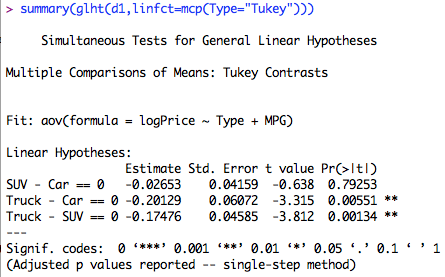
\includegraphics[scale=0.5]{d1tukey}
\end{center}
The output shows that the logged prices of trucks are significantly lower than cars and SUVs. SUVs and cars do not have a significant difference. One may think of it as trucks being in one group, and SUV and car are in another another group.
\section{Regression Diagnostics}
Regression diagnostics check assumptions.
\begin{center}
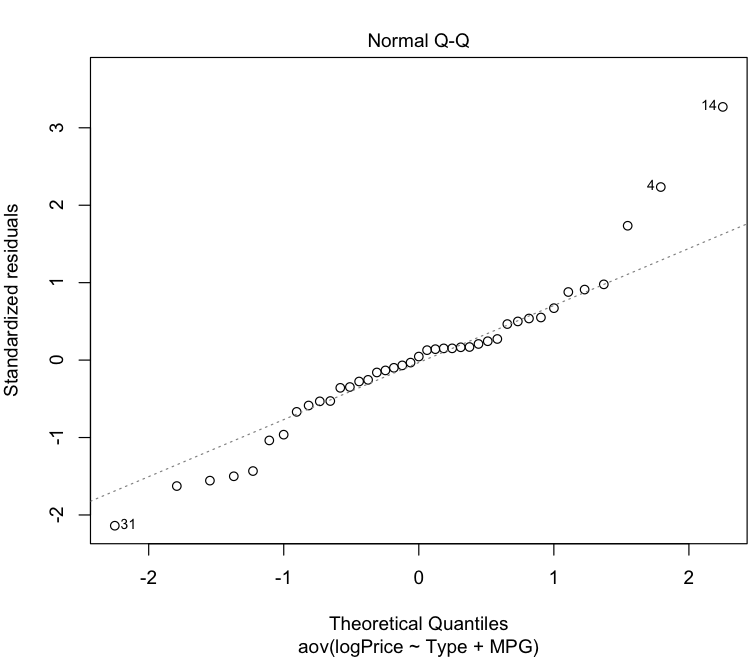
\includegraphics[scale=0.3]{diagqq}
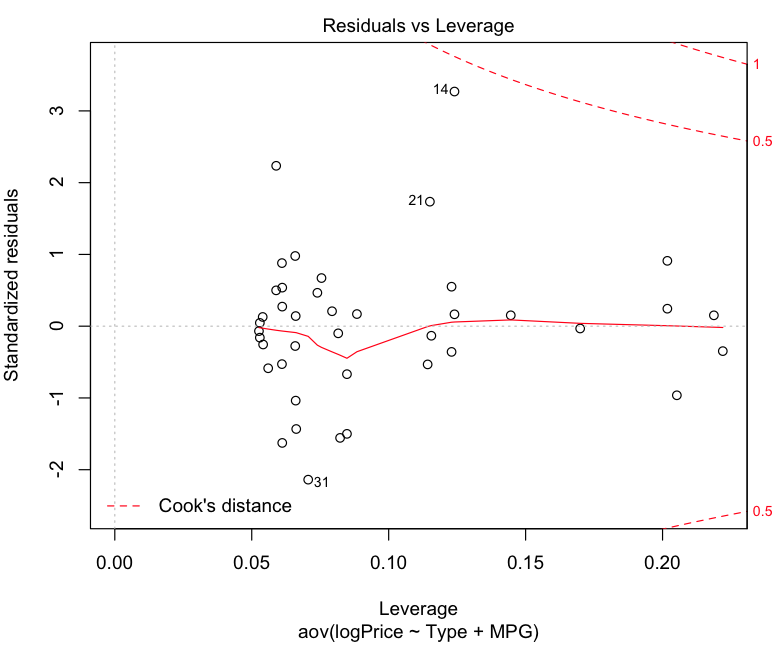
\includegraphics[scale=0.3]{diagstd}
\end{center}
QQ plot shows that there are a few outliers above the line to the far right. There are also some points below the lines to the far left.

We expect 95\% of the points lie within $\pm 2.5$ standard residuals band. Observation 14 lies outside this range.

Cook's distance measures influence. One should expect Cook's distance to be less than 1. The plot shows that all points lie within this range (shown by the dotted curves marked by 1).

A good guideline for what constitutes as a large leverage value is $2.5\left( \frac{p+1}{n}\right) = 2.5 \left( \frac{3+1}{41}\right) = 0.098$. Almost half of the data points have leverage greater than this value. A detailed output is provided below.
\begin{center}
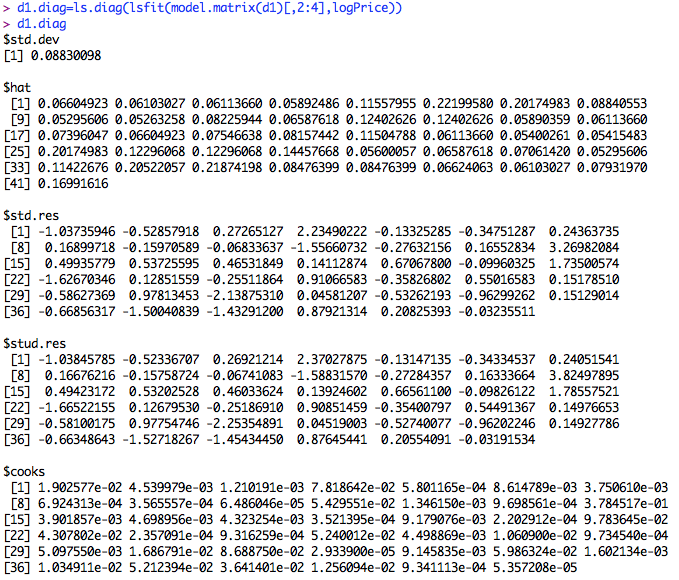
\includegraphics[scale=0.5]{diag1}
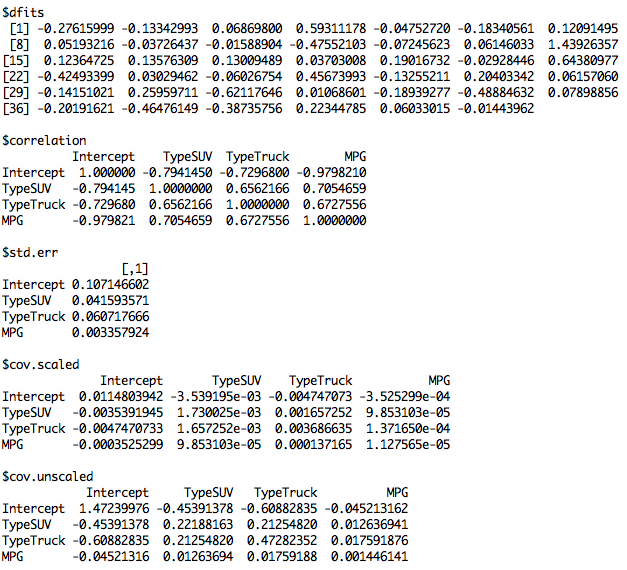
\includegraphics[scale=0.5]{diag2}
\end{center}
Observation 14 has a standard residual of 3.82. It is Toyota Land Cruiser, an SUV with 15.5 MPG costing \$79,605. The points that have high leverage values are observation 5(0.11557955), 6(0.22199580), 7(0.20174983), 13(0.12402626), 14(0.12402626), 21(0.11504788), 25(0.20174983), 26(0.12296068), 27(0.12296068), 28(0.14457668), 33(0.11422676), 34(0.20522057), 35(0.21874198), and 41(0.16991616). These points are Toyota Sienna, Toyota Tacoma, Toyota Tundra, Toyota Sequoia, Toyota Land Cruiser, Honda CRZ, Honda Ridgeline, Nissan Juke, Nissan Rogue, Nissan Rogue Select, Nissan Armada, Nissan Frontier, Nissan Titan, and Nissan Maxima, respectively.

Most vehicles have border line leverage value, around 0.10. The ones have very high leverage values, say, around 0.20, are all trucks. This is expected as we only have five trucks in the data. There is nothing to do about them. Taking out these points is not really something we want to do, since that is taking out an entire level in the variable type.

Below are a side-by-side box plot of Type versus standard residuals and a plot of MPG versus standard residuals.
\begin{center}
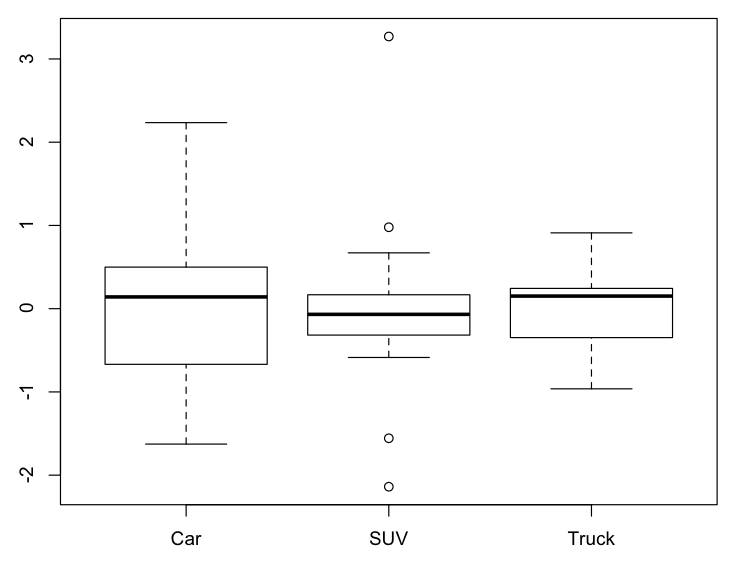
\includegraphics[scale=0.3]{diagbox}
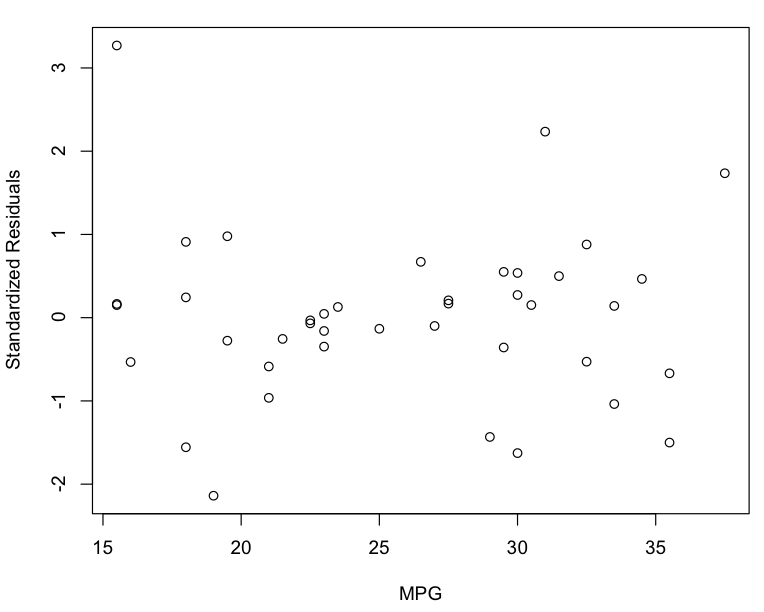
\includegraphics[scale=0.3]{diagscat}
\end{center}
Toyota Land Cruiser, the SUV with standard residual of 3.82 is apparent in the side-by-side box plots and far left in the MPG versus standard residuals plot. We can see that cars have more variability than SUVs and trucks, but its residuals lie within $\pm 2.5$ range. We will later check with Levene's test to see if there is non-constant variance. The plot of MPG versus standard residuals looks okay.

Below is the output of Levene's test.
\begin{center}
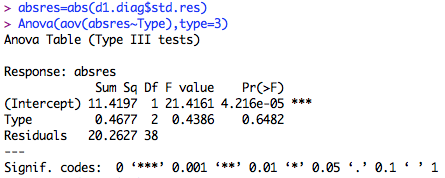
\includegraphics[scale=0.5]{diaglevene}
\end{center}
The $F$-statistics is 0.4386, giving a $p$-value of 0.6482. The test is not significant, so non-constant variance is addressed after we took log.
\section{Prediction Interval}
Below is
Our regression model allows us to write down a model for prediction. The predicted price for a certain type of vehicle $i$ with $x$ MPG equals
\[
\text{Least Squares Mean}_i + \hat \beta_1(x - \bar x)
\]
$\bar x$ is the means of MPG, which in this case is 25.73171. Let us predict the price of a truck with 20 MPG. It has logged price
\[
4.223206 + (-0.022747)(20-25.73171) = 4.35358520737
\]
or $10^4.35358520737 = \$22573$ after anti-logging. A rough prediction 95\% interval is calculated as
\[
4.35358520737 \pm 2 \times 0.0883 = (4.157499,4.549673)
\]
\begin{center}
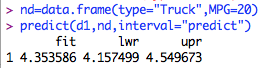
\includegraphics[scale=0.6]{d1pred}
\end{center}
or (14371,35455) in the original scale.
\section{Adding an Interaction}
The above model does not include an interaction effect. Here, we investigate whether different slopes for MPG for each type of automobile would improve the model. Below are the output of the regression.
\begin{center}
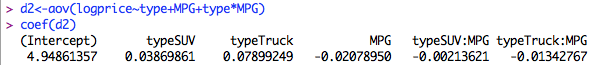
\includegraphics[scale=0.5]{d2a} \\
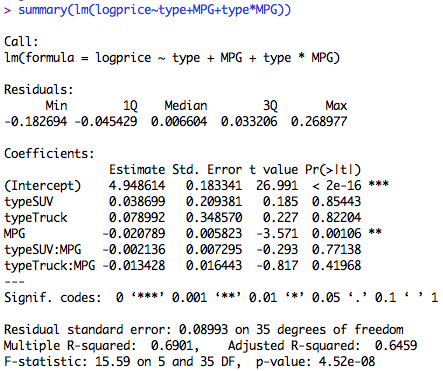
\includegraphics[scale=0.5]{d2b} \\
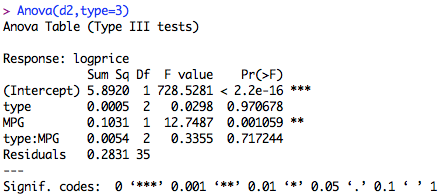
\includegraphics[scale=0.5]{d2c}
\end{center}
Notice that type : MPG has an F value of 0.3355, which gives $p$-value of 0.717244, not statistically significant at all. Adding the interaction of type of automobile and MPG does not help.

The $t$-test for typeSUV:MPG shows that the coefficient for typeSUV is not significantly different from the overall coefficient for the variable Type, as it has a $p$-value of 0.77138. The $t$-test for typeTruck:MPG is not significant either.

The missing coefficient for typeCar:MPG is calculated as $0-(-0.002136 - 0.013428) = 0.01556388$ since their coefficient must sum to zero.

This model that includes the interaction effect between type of vehicle and MPG corresponds to separate regression line for each type of automobile. We plot separate lines on the same plot below
\begin{center}
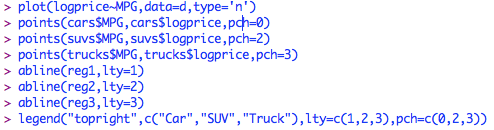
\includegraphics[scale=0.5]{plot} \\
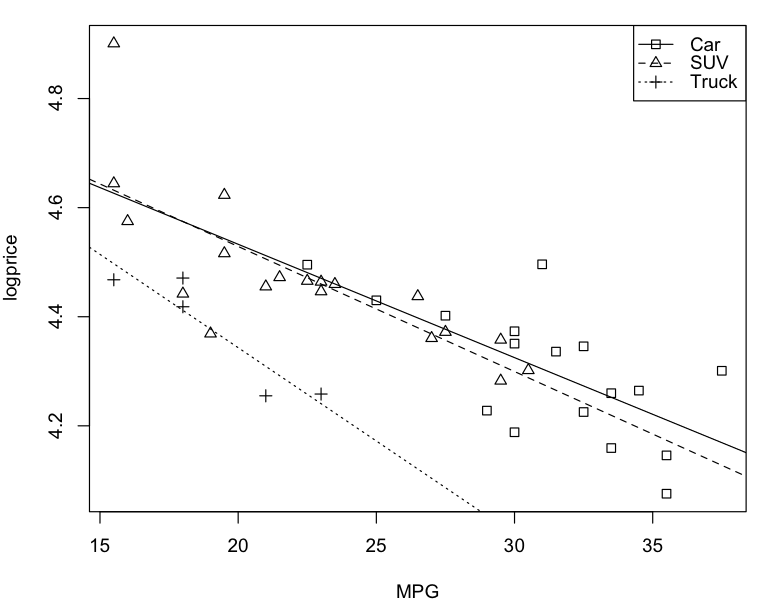
\includegraphics[scale=0.3]{plot1}
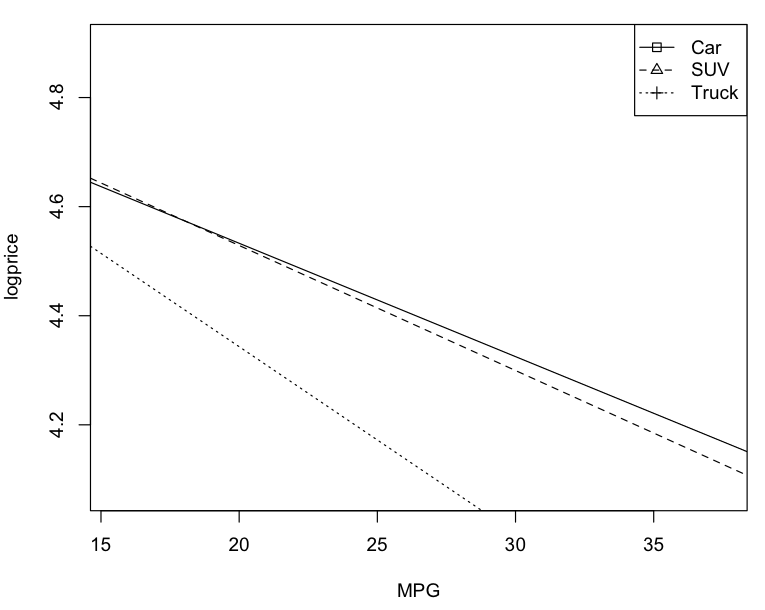
\includegraphics[scale=0.3]{plot2}
\end{center}
Notice that the slopes are fairly parallel, with the exception of trucks having a steeper slopes.
\section{Conclusion}
In this analysis, we conducted an ANCOVA model of price of vehicles built by three major Japanese automakers based on one categorical, one numerical variable--type of vehicles and MPG, respectively. By examining price versus type box plot, cars have the least price, followed by trucks and SUVs. Interestingly, the least squares means show that given MPG, trucks cost the least, followed by SUVs, then cars.

Finally, interaction effect between type and MPG is not significant.
\end{document}